%!TeX program = xelatex
\PassOptionsToPackage{quiet}{fontspec}
\documentclass[10.5pt,compsoc,UTF8]{CjC}
\usepackage{thesis}
%===============================%信息设置
\mycourse{《test》}
\mytitle{如何正确高效地摸鱼}
\myauthor{PhilFan}
\mystudentid{19260817}
\myschool{XX学院}
\myteacher{PhilFan}

\begin{document}
\setpage

\Title{\themytitle}{\themyauthor}{\themystudentid}

\myabstract{
\zhlipsum[5]
}
\vspace {5mm}
\keyword{摸鱼；LaTeX}


\vskip 45mm

\begin{center}
\zihao{3}{ \bf LaTeX on Overleaf}\\
\vspace {5mm}

\end{center}

\zihao{5}{\noindent
{\bf Abstract}\quad 
\zihao{5}{\noindent \lipsum[5]
\par}}
\vspace {5mm}
{\noindent{\bf Keywords}\quad LaTeX}


% 正文
\clearpage
\section{引言}

\begin{table}[htbp]
  \centering
    \begin{tabular}{ccp{20em}}
    \toprule
    编号    & 仪器用具名称     & 主要参数（型号，测量范围，测量精度等） \\
    \midrule
    1	&	数字万用表\\
    2	&	直流稳压电源\\
    3	&	电子技术实验箱\\
    4	&	示波器\\
    5	&	函数信号发生器\\
        6   &	运放LM358\\
    \bottomrule
    \end{tabular}%
  \label{tab:devicehttps://cn.overleaf.com/project/6a048745e789debfee07edab}%
  \caption{我是一个表格}
\end{table}%

\section{第一节}
\zhlipsum[5]
\begin{figure}[!htbp]
    \centering
    \begin{minipage}[b]{0.45\linewidth}
        \centering
        
\includegraphics[width=0.9\textwidth]{example}
        \caption{非子图并排题注1}
         
    \end{minipage}%
    \begin{minipage}[b]{0.45\linewidth}
        \centering
        
\includegraphics[width=0.9\textwidth]{example}
        \caption{非子图并排题注2}
         
    \end{minipage}
\end{figure}


\section{第二节}


\zhlipsum[5] % 生成随机文字

杭州不要再下雨啦，我知道你有你的烦恼，但我们也期盼着能有更多的阳光洒满这座美丽的城市。虽然雨水能带来生机和活力，但持续的阴雨天气也会让人感到压抑和沉闷。让我们一起期待阳光的到来，让杭州的天空重新焕发出明亮的光彩。同时，也希望大家在雨天注意出行安全，照顾好自己和身边的人。

\begin{figure}
    \centering
    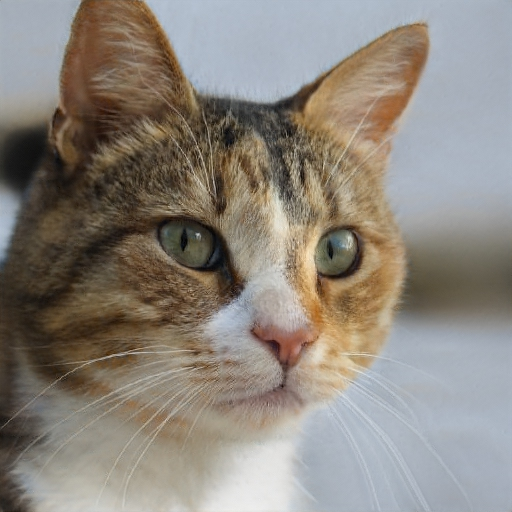
\includegraphics[width=0.5\linewidth]{figures/example.png}
    \caption{Enter Caption}
    \label{fig:enter-label}
\end{figure}


\newpage
\section{代码展示}
\begin{problem}
adsfa
\end{problem}
\begin{solution}
\end{solution}
\begin{lstlisting}[language=Python, caption=Python example]
def hello_world():
    print("Hello, world!")
\end{lstlisting}


% 参考文献
\clearpage
\reference
\end{document}


